
\documentclass[14pt]{extarticle}
\usepackage{graphicx}
\usepackage[margin=1in]{geometry}

\graphicspath{ {./images/} }

\begin{document}
    \pagenumbering{arabic}
    \pagestyle{plain}

    \title{\Huge Assignment 1\\ Computer Networks}
    \author{\huge Vikas Gola}
    \maketitle
    \newpage

    \noindent
    \textbf{\large Question 1}
    What are the network interfaces available on your computer? Which network did you
    eventually select in your experiments.\\[10pt]
    \textbf{\large Answer}
    The following network interfaces are available
    \begin{itemize}
        \item enp2s0
        \item any
        \item Loopback:io
        \item wlp3s0b1
        \item bluetooth0
        \item nflog
        \item nfqueue
        \item usbmon1
        \item usbmon2
    \end{itemize}
    enp2s0 network interface is selected\\[8pt]
    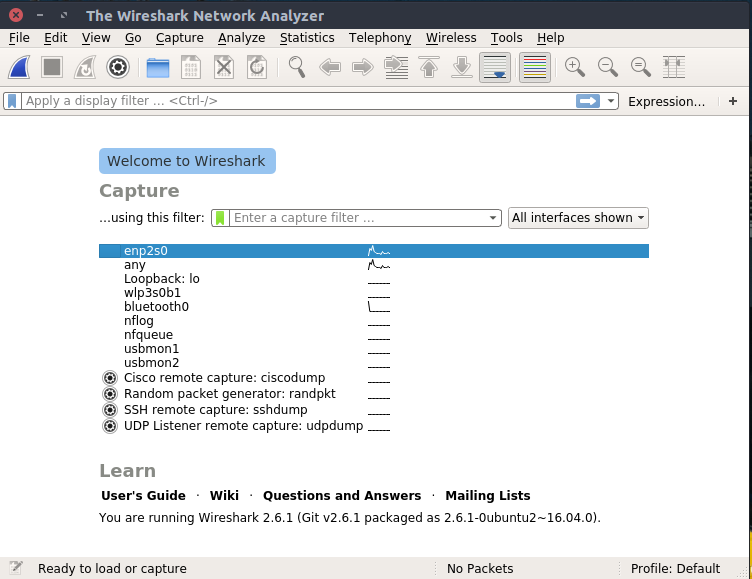
\includegraphics[scale=0.55]{1}
    \vspace{1cm}
    
    \noindent
    \textbf{\large Question 2}
    Which application layer protocol is used in this case?\\[10pt]
    \textbf{\large Answer}
    HyperText Transfer Protocol(HTTP).\\[8pt]
    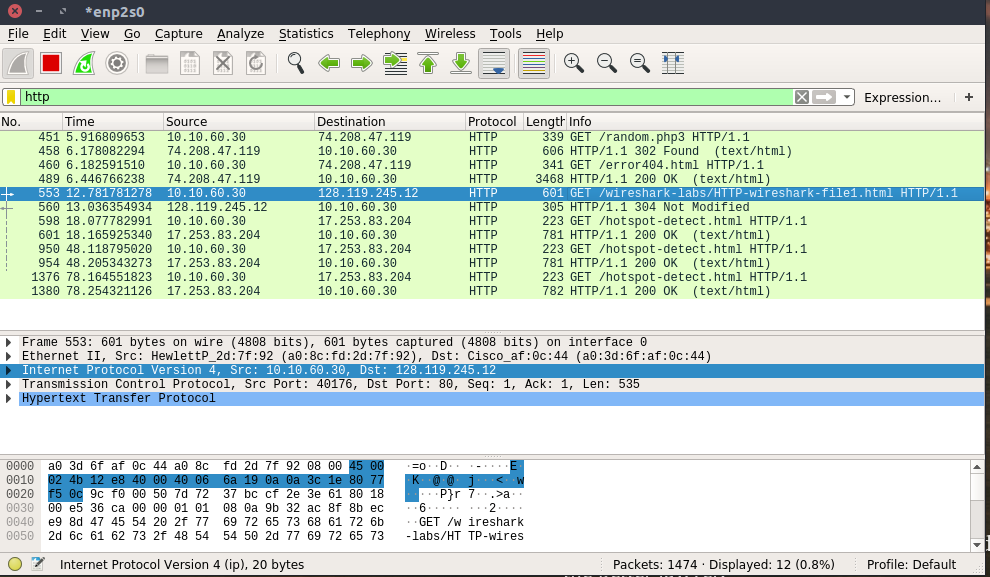
\includegraphics[scale=0.45]{2}
    \vspace{1cm}


    \noindent
    \textbf{\large Question 3}
    What are the other protocols used and displayed in the unfiltered packet listing window of
    wireshark, besides the one that you answered in Q2?\\[10pt]
    \textbf{\large Answer}
    The other protocols in unfiltered packet listing windows are
    \begin{itemize}
        \item UDP
        \item TLS
        \item CDP
        \item TCP
        \item ARP
        \item STP
        \item SSDP
        \item DNS
        \item MDNS
        \item NBNS
        \item LLMNR
        \item DHCP
    \end{itemize}
    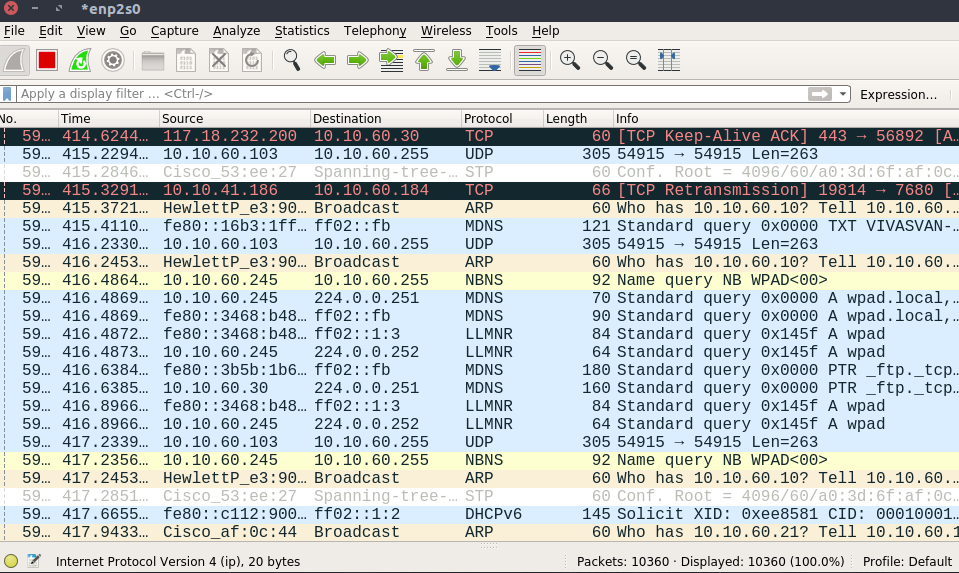
\includegraphics[scale=0.45]{3}
    \vspace{1cm}


    \noindent
    \textbf{\large Question 4}
    What is the IPA of your machine? What is the IPA of the destination machine? Is there any
    way by which you can ascertain that the IPA of the destination indeed is the same as that
    you observed in wireshark? If so, how ?\\[10pt]
    \textbf{\large Answer}
    IPA of my machine is 10.10.60.30. IP address of destination is 128.119.245.12. 
    IPA of destination can be verified by using the ping on the host of website which is \textbf{gaia.cs.umass.edu}.\\
    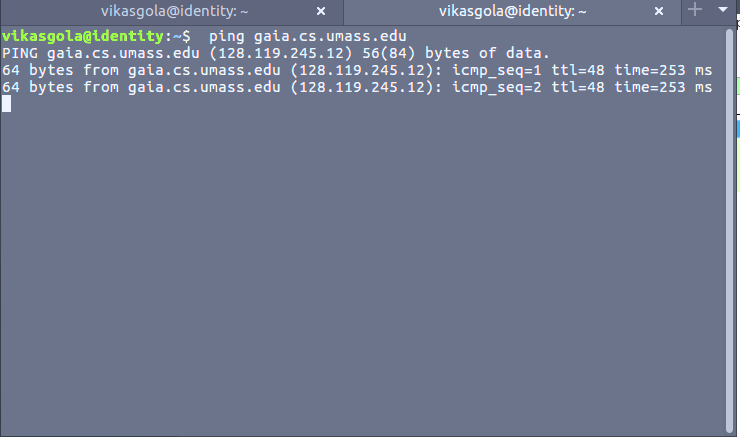
\includegraphics[scale=0.6]{4}
    \vspace{1cm}

    \noindent
    \textbf{\large Question 5}
    What is the class of the IPA of the source machine ? That of destination machine?\\[10pt]
    \textbf{\large Answer}
    class A, class B
    \vspace{1cm}

    \noindent
    \textbf{\large Question 6}
    How many bits were captured in this packet? At what time was this packet captured?\\[10pt]
    \textbf{\large Answer}
    490 bytes were captured in this packet on date Aug 20,2018 at time 02:39:42.595559043 IST.\\[10pt]
    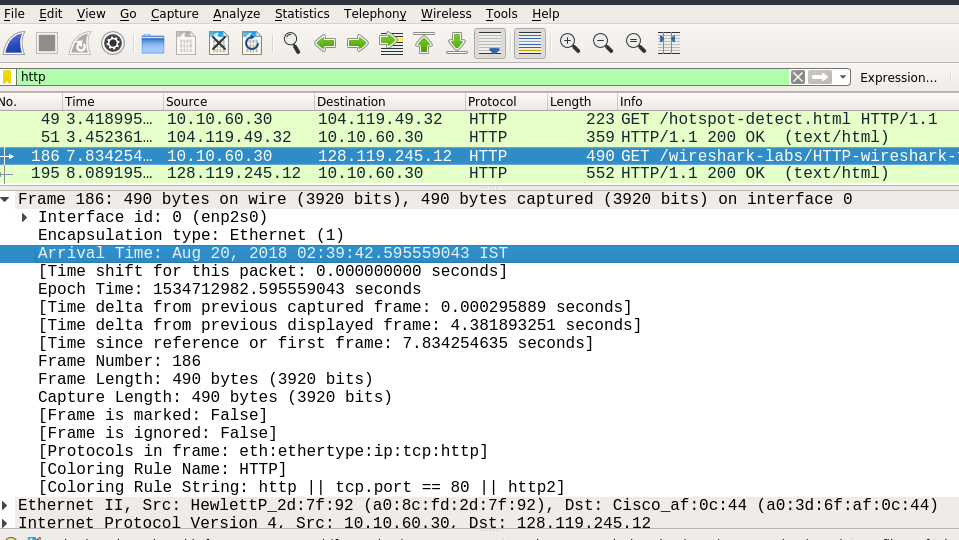
\includegraphics[scale=0.48]{6}
    \vspace{1cm}

    \noindent
    \textbf{\large Question 7}
    What is the interface id used? What is the address of the interface?\\[10pt]
    \textbf{\large Answer}
    Interface id is 0 (enp2s0) and address of this interface is a0:8c:fd:2d:7f:92.\\[10pt]
    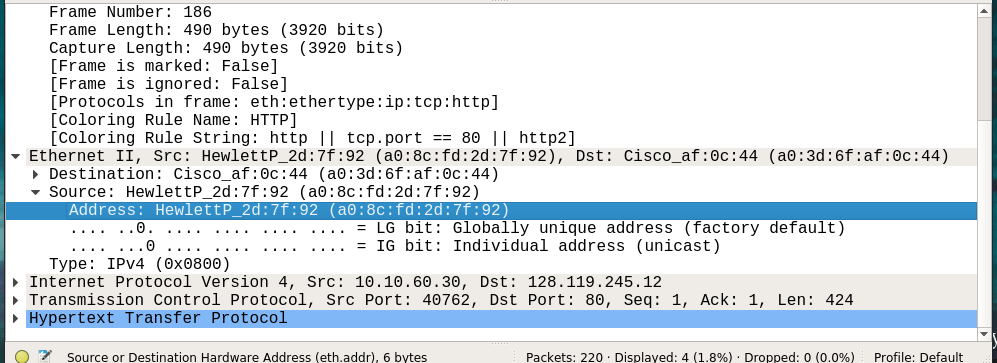
\includegraphics[scale=0.48]{7}
    \vspace{1cm}

    \noindent
    \textbf{\large Question 8}
    How long did it take from when the HTTP GET message was sent until the HTTP OK reply was
received? (By default, the value of the Time column in the packet-listing window is the
amount of time, in seconds, since Wireshark tracing began. To display the Time field in time-
of-day format, select the Wireshark View pull down menu, then select Time Display Format,
then select Time-of-day.)\\[10pt]
    \textbf{\large Answer}
    HTTP GET message was sent at 02:39:42.595559043 IST and HTTP OK was received at 02:39:42.850499547 IST.\\[8pt]
    Time taken = received time - sent time \\= 42.850499547 - 42.595559043 \\
    = 0.254940504 seconds.\\[10pt]
    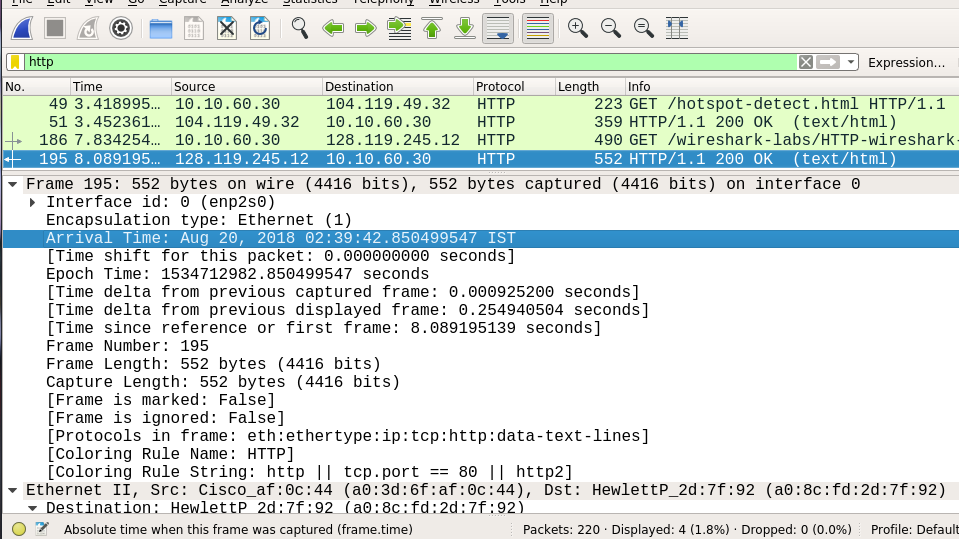
\includegraphics[scale=0.48]{8}
    \vspace{1cm}

    \noindent
    \textbf{\large Question 10}
    Print the two HTTP messages (GET and OK) referred to in question above. To do so, select
Print from the Wireshark File command menu, and select the "Selected Packet Only" and
"Print as displayed" radial buttons, and then click OK.\\[10pt]
    \textbf{\large Answer}
    HTTP GET message and OK message can be checked at last of the pdf file respectively.
    \vspace{1cm}

    \noindent
    \textbf{\large Question 11}
    What is the destination physical address of the first packet captured? What device does it
belong to? Show where in the capture would you find this information.\\[10pt]
    \textbf{\large Answer}
    Physical address of the destination in the first packet is 
    a0:3d:6f:af:0c:44 which is find in the destination tab of \textmd{Ethernet Block}.\\[10pt]
    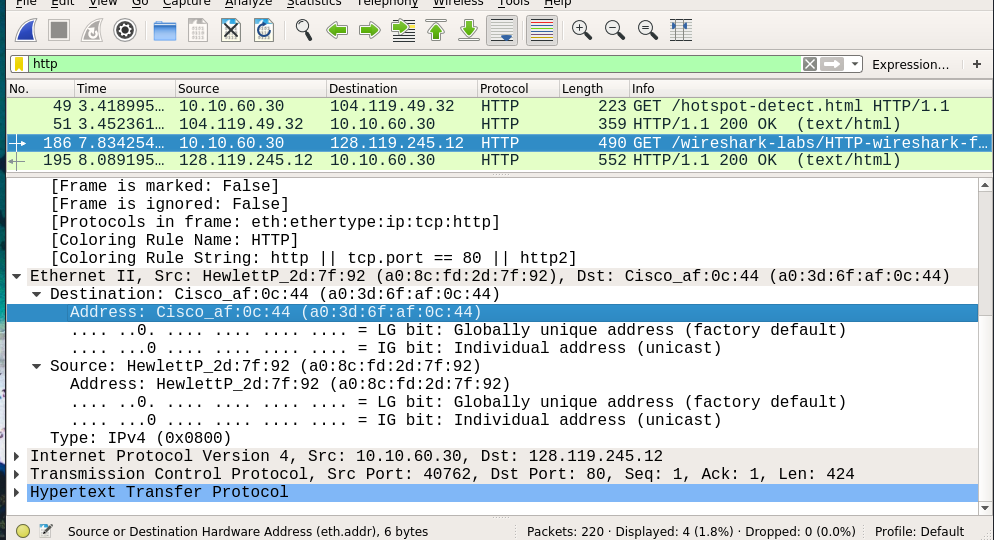
\includegraphics[scale=0.5]{11}
    \vspace{1cm}
    
    \noindent
    \textbf{\large Question 12}
    How many bytes of header does the first frame sent have? Show where in the capture would
you find this information.\\[10pt]
    \textbf{\large Answer}
    20 bytes of header have been sent and this information is find in Internet Protocol Version 4 block.\\[10pt]
    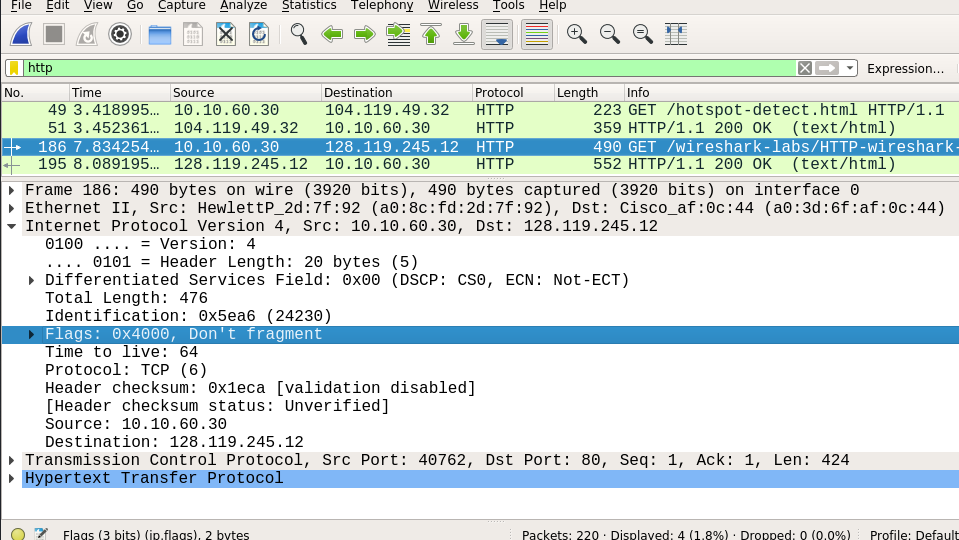
\includegraphics[scale=0.45]{12}
    \vspace{1cm}
    
    \noindent
    \textbf{\large Question 13}
    By looking at the Ethernet header of a frame, can we determine if it contains an IP packet?
Show where in the capture would you find this information.\\[10pt]
    \textbf{\large Answer}
    Yes, we can easily determine it by looking at the "type" in Ethernet header of a frame.
    \vspace{1cm}
    
    \noindent
    \textbf{\large Question 14}
    Is it possible to know if the first packet captured has TCP or UDP as transport protocol by
looking at the IP header? Explain and show where in the capture would you find this
information.\\[10pt]
    \textbf{\large Answer}
    Yes, it is possible to find the transport protocol type of first captured packet 
    which is visible in IP header written as "Protocol: TCP" indicates the TCP transport protocol.\\[10pt]
    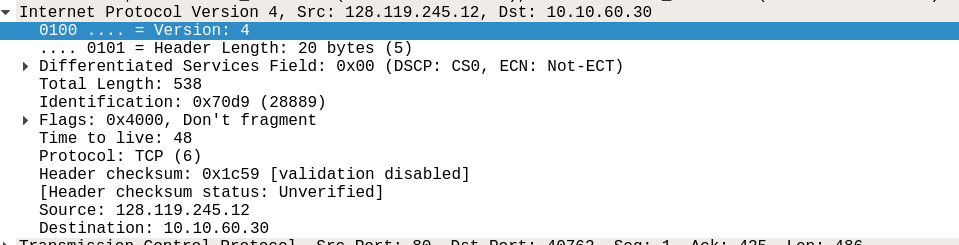
\includegraphics[scale=0.5]{14}
    \vspace{1cm}
    
    \noindent
    \textbf{\large Question 15}
    In the SYN, ACK. What are the source and destination ports? Are these the same for the
client and the server? Explain why.\\[10pt]
    \textbf{\large Answer}
    Source Port: 40762 and Destination Port:80\\
    No, these are not same for client and server as same port indicates same process 
    and also there are some fix ports for handling specific type requests.
    \vspace{1cm}

    \noindent
    \textbf{\large Question 16}
    Why does the Server Hello message sent by the server have 1 as a relative sequence number
and 185 as a relative acknowledgement number.\\[10pt]
    \textbf{\large Answer}
    Wireshark always displayed a SYN(Sequence) and ACK(Acknowledgement) number relative to the first seen segment for that conversation. 
    That’s why all SYN and ACK numbers always startat 0 for the first packet seen in each conversation.
    After setting up the connection between client and server, when server start transmitting data,relative ACK number is equal to (Bytes sent +1). 
    That’s why in this example, relative SEQnumber is 1 and relative ACK is (184+1=185), because packet sent till Server Hello message are 184. \\[10pt]
    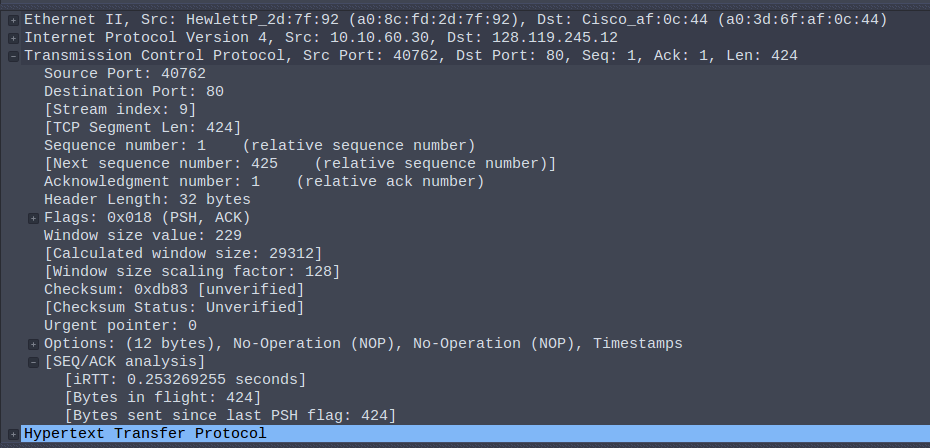
\includegraphics[scale=0.5]{16}
    \vspace{1cm}

    \noindent
    \textbf{\large Question 17}
    What is the first sequence number sent by the server to the client. Why is it not the 0
displayed by wireshark?\\[10pt]
    \textbf{\large Answer}
    As explained in answer of last question, Wireshark always displayed a SYN(Sequence) and ACK(Acknowledgement) number relative to the first seen segment for that conversation.
    Because, client has already sent some packets to server and hence packets sent by server is not the first in communication and it's not 0. \\[10pt]
    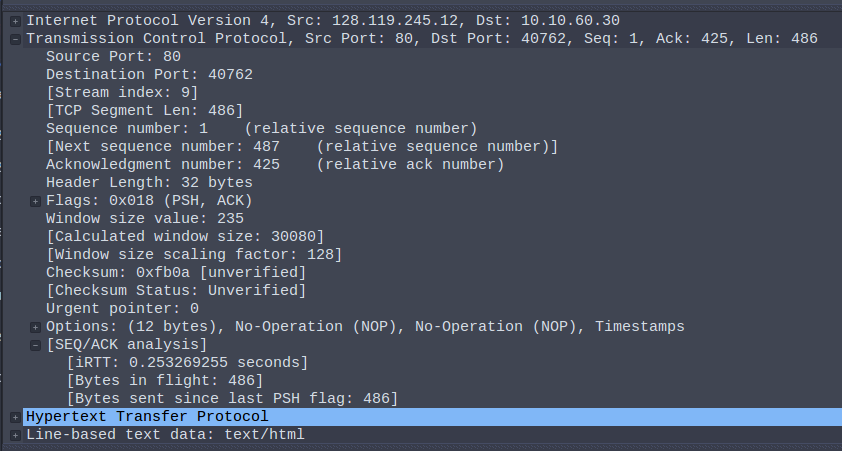
\includegraphics[scale=0.5]{17}
    \vspace{1cm}
    
    
\end{document}